\documentclass[12pt]{article}

\usepackage[utf8]{inputenc}	    %input

\usepackage{amsfonts,amssymb,amssymb,amsmath}% math packages
\allowdisplaybreaks[1]
\usepackage[ruled]{algorithm2e} %algorithm package
\usepackage[title,toc,titletoc]{appendix}
\usepackage{autobreak}
\usepackage[english]{babel}		%for other languages
% bibliographic package
\usepackage[backend=biber, style=apa6, doi=true]{biblatex}
\DeclareFieldFormat{titlecase}{#1}
\AtBeginBibliography{%
  \urlstyle{sf}%
}
\usepackage{blindtext}
\usepackage[font=small,labelfont=bf]{caption}
\usepackage{color}
\usepackage{csquotes}           %for quote environment
\usepackage{dsfont}
\usepackage{enumitem}			%list environment
\usepackage{float}              %for image floating
\usepackage[T1]{fontenc}		%output
\usepackage[top= 1 in, bottom= 1 in, left= 1 in, right= 1 in]{geometry}				%margin manipulation
\usepackage[bottom]{footmisc}
\usepackage{graphicx}           %for image  
\usepackage[colorlinks=true,urlcolor=blue]{hyperref}
\usepackage{lmodern}    	    %latin modern font
\usepackage{longtable}
\usepackage[pagewise,mathlines]{lineno}
%\linenumbers
\usepackage{makecell}
\usepackage{mathtools}
\usepackage{marvosym}	        %symbols in contact information
\usepackage{minted}
\usepackage{parskip}
% no indent with single paragraph spacing
\setlength{\parindent}{0pt}
\setlength{\parskip}{0 pt}
\setlength{\footnotesep}{\baselineskip}
\setlength {\marginparwidth}{2cm} 
% overall spacing of the contents
\usepackage{setspace}
\linespread{1.15}
\usepackage{soul}
\usepackage{titlesec}
\titleformat*{\section}{\large\bfseries}
\titleformat*{\subsection}{\large\bfseries}
\titleformat*{\subsubsection}{\normalsize\bfseries}
\usepackage{verbatim}	        %comment environment
\usepackage[dvipsnames]{xcolor}

\usepackage{xurl}
\urlstyle{tt}

% listing package definition
\usepackage{listings}
\lstdefinestyle{terminal}{columns=fullflexible,
keepspaces=true,
breaklines=true,
basicstyle={\footnotesize\fontfamily{fvm}\fontseries{m}\selectfont},
keywordstyle={\footnotesize\fontfamily{fvm}\fontseries{b}\selectfont},
commentstyle={\color{comments}\small\fontfamily{fvm}\itshape\selectfont},
frame=single,
xleftmargin=0in,
backgroundcolor=\color{lightgray!50},
belowcaptionskip=10pt,
aboveskip=0.5cm}
\lstset{style=terminal,float=h,language=bash}

\newcommand{\fenics}{\textsf{FEniCS}}
\newcommand{\fenicsx}{\textsf{FEniCSx}}


\graphicspath{{fenicsx_figures/}}

\begin{document}

\begin{center}
    {\textbf{\Large Getting started with \fenicsx}}\\ \vspace{0.25 cm}
    Bibekananda Datta \\
    Department of Mechanical Engineering, Johns Hopkins University, Baltimore, MD \\ \vspace{0.25 cm}
    March 2023
\end{center}
\vspace{5 mm}
\hrule

\section*{What is \fenicsx}

\fenicsx\ is an open-source multi-platform computing environment to solve partial differential equations using the finite element method. \fenicsx \ supports parallel computing with Python and C++ interface. \fenicsx \ is comprised of the libraries UFL, Basix, FFCx, and DOLFINx which are the build blocks of it. To learn more about \fenicsx: \url{https://fenicsproject.org}.

\begin{figure} [H]
    \centering
    
\includegraphics[width=2cm]{fenics-logo.png}
\end{figure}

The \fenics \ project originally started in 2003 and was known as \fenics. In 2020, the developers released a new version of the library and renamed \fenics \ as \fenicsx. The latest stable version of legacy \fenics \ was released in April 2019 and it's barely updated. But many tutorials and legacy codes are perhaps written in legacy \fenics. So you may want to install a version of it. We will demonstrate installing both versions on multiple different platforms here.

\begin{figure} [H]
    \centering
    
\includegraphics[width=7cm,trim={0 3.5cm 0 3.5cm},clip]{all-os-logo.png}
\end{figure}

Both \fenicsx \ and \fenics \ are available on Linux, macOS, and Windows. You can download and install it in different ways. Check out the options here for \fenicsx: \url{https://github.com/FEniCS/dolfinx} and here for legacy \fenics: \url{https://fenicsproject.org/download/archive/}. For both versions, our preferred approach is to install them via Anaconda.


\section*{Installation on Windows} 

This step is only applicable if you are using Windows. You will have to set up Windows Subsystem for Linux (WSL) to use Anaconda-based installation of \fenicsx \ and legacy \fenics. WSL is a virtual Linux environment within Windows that allows you to use Linux command line tools and GUI applications (GUI is natively supported on Windows 11). If you are on macOS or Linux, you can skip this step. If you are on Windows and already have installed WSL, it still might be interesting to download the recommended applications/ tools, such as VS Code.

\subsection*{Get your tools ready first}

\subsubsection*{PowerShell 7}

Microsoft Windows already comes with Windows PowerShell 5.1, but the modern edition of PowerShell 7 is more powerful and available on different operating systems. 

\begin{figure}[H]
    \centering
    
\includegraphics[width=2.5cm,trim={0 1.5cm 0 1.5cm},clip]{powershell-logo.png}
\end{figure}
To learn more about this, check this:
\url{https://learn.microsoft.com/en-us/powershell/scripting/install/installing-powershell-on-windows}.

\begin{enumerate}[label={\arabic*.}, leftmargin= 0.6 cm,itemsep = 0.25cm,topsep= .25cm]

\item Install the App Installer from the Microsoft App Store. That will enable the \texttt{winget} tool on default PowerShell 5.1 and new PowerShell 7.X.Y to be installed.

\item Open the default Windows PowerShell 5.1 as \textbf{administrator} from the Windows Start menu, then do the following:

\begin{lstlisting}[style=terminal]
$ winget search Microsoft.PowerShell
\end{lstlisting}

This command will return the available PowerShell versions to install. We do not recommend installing the \texttt{.preview} version. 

\item Now install the stable release of PowerShell using the following command:

\begin{lstlisting}[style=terminal]
$ winget install --id Microsoft.Powershell --source winget
\end{lstlisting}

\end{enumerate}

\subsubsection*{Windows Terminal} 

Windows Terminal is a command line tool, available on \textbf{Microsoft Store} (\url{https://apps.microsoft.com/store/apps}). You can manage multiple command line environments such as Windows PowerShell 5.1, PowerShell 7.X.Y, CMD, WSL, etc. using a single application.

\begin{figure}[H]
    \centering
    
\includegraphics[width=2.5cm,trim={0 1cm 0 1.5cm},clip]{terminal-logo.png}
\end{figure}

Check out more about it here: \url{https://learn.microsoft.com/en-us/windows/terminal/install}. You can customize your command line applications using Terminal.

\subsection*{Windows Subsystem for Linux (WSL)}

\begin{enumerate}[label={\arabic*.}, leftmargin= 0.6 cm,itemsep = 0.25cm,topsep= .25cm]

\item The current stable version for Windows Subsystem for Linux is WSL2 and this is the default installation. Open PowerShell 7.X.Y (your current installation version) as \textbf{administrator} using the Terminal app from the Windows Start menu and then type the following command:
\begin{lstlisting}[style=terminal]
$ wsl --list --online
\end{lstlisting}
This command will show you currently available Linux distributions on Windows. 

\item Install the latest LTS version of Ubuntu which is Ubuntu 22.04.02 LTS.

\begin{lstlisting}[style=terminal]
$ wsl --install -d Ubuntu
\end{lstlisting}
It will ask you to create a user account and set a password. The installation process is fast and straightforward. 

\item Once Ubuntu in WSL is installed, you can use it similarly to a regular Ubuntu distribution. To run Ubuntu, open it from the Terminal application option. If this is your first time using Linux, you can familiarize yourself with some commands and operations from here: \url{https://ubuntu.com/tutorials/command-line-for-beginners}.

\item We will now update the Ubuntu distribution and install two packages for WSL virtual display settings.

\begin{lstlisting}[style=terminal]
$ sudo apt update && sudo apt upgrade
$ sudo apt install xvfb libgl1-mesa-glx
\end{lstlisting}

The first command will ask for your password. Proceed as needed.

\item To open Windows like File Explorer from Ubuntu, type:
\begin{lstlisting}[style=terminal]
$ explorer.exe .
\end{lstlisting}

You can open the WSL home directory and browse, copy, and move files like Windows.

\item Once you have installed Ubuntu in WSL and VS Code, you can follow these tutorials to get yourself more familiarized with the VS Code environments and capabilities in WSL:
\url{https://learn.microsoft.com/en-us/windows/wsl/tutorials/wsl-vscode} and \url{https://code.visualstudio.com/docs/remote/wsl-tutorial}.

\item To use packages and libraries installed in WSL, start VS Code from the Ubuntu terminal.

\end{enumerate}

\section*{Anaconda on Linux (WSL) and macOS}

If this is the first time you are using Python, then sit back, it is going to get confusing like this xkcd comic. Even if you are experienced in Python, you might find this interesting.\\

\begin{figure}[ht]
    \centering
    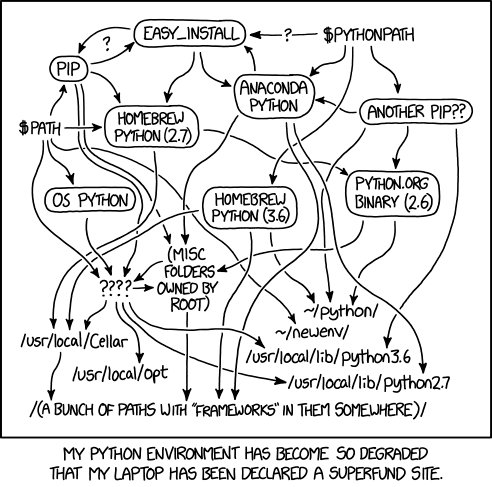
\includegraphics[width=8cm]{xkcd-python.png}
\end{figure}

Most of the Python-based libraries and packages often depend on other libraries and packages (called dependencies). Installing the right version of those packages and maintaining them is often a complex task even for experienced developers. So, we will use a popular Python distribution, Anaconda, to manage all the Python-based libraries and relevant dependencies. Anaconda uses the conda package manager and works well with pip (Python's default package manager). Installation of Anaconda comes with popular Python packages such as NumPy, SciPy, Matplotlib, and <\emph{insert hundred other packages here}>. It also comes with Jupyter Notebook and Spyder IDE. Anaconda also has a minimalist version, called Miniconda, which is lightweight because it only includes the conda manager and a few packages. We strongly recommend installing Anaconda.

\begin{figure}[H]
    \centering
    
\includegraphics[width=6cm]{anaconda-logo.png}
\end{figure}

\begin{enumerate}[label={\arabic*.}, leftmargin= 0.6 cm,itemsep = 0.25cm,topsep= .25cm]


\item This step is only for macOS. We will install \texttt{xcode} command line tools to enable basic development libraries and features. On the macOS terminal, type:

\begin{lstlisting}[style=terminal]
(base) $ xcode-select --install
\end{lstlisting}


\item Download Anaconda from here based on your operating system and architecture: \url{https://www.anaconda.com/products/distribution}.

\item On macOS, you can download the graphical installer and install it like every other software by following the on-screen instructions. Details of the installation procedure are available here: \url{https://docs.anaconda.com/anaconda/install/mac-os/}. Alternatively, you can download the installation script and use the command line to install Anaconda like Linux.

\item For WSL, you will download the installation script. Open the Ubuntu terminal and use the following command to copy this script from your Windows Downloads folder to WSL home directory:

\begin{lstlisting}[style=terminal]
$ wget https://repo.anaconda.com/archive/Anaconda3-2023.03-Linux-x86_64.sh
\end{lstlisting}

\texttt{Anaconda3-2023.03-Linux-x86\_644} is the latest version of Anaconda available at the time this guide is being written. Check the available versions here: \url{https://repo.anaconda.com/archive}. Replace it with the version you downloaded for installation.

\item Once it is copied into the home directory, you can run the following command on the Ubuntu terminal for installation:

\begin{lstlisting}[style=terminal]
$ bash Anaconda3-2022.10-Linux-x86_64.sh
\end{lstlisting}

Please make sure to use the version you downloaded. It will ask you to read the license agreement and your permission for installation. Proceed as needed.

\item Close the Ubuntu terminal and open it back, you will see the base environment for Anaconda is now available. This is how your terminal is going to look like:
\begin{lstlisting}[style=terminal]
(base) $ 
\end{lstlisting}

\item Check out these operations and commands for using Conda: \url{https://docs.conda.io/projects/conda/en/4.6.0/_downloads/52a95608c49671267e40c689e0bc00ca/conda-cheatsheet.pdf}

\end{enumerate}

\section*{\fenicsx \ on Linux and macOS}

As of March 2023, the latest stable release of \texttt{dolfinx} available via Anaconda is 0.6. If you build \fenicsx \ from the source, you can perhaps install 0.7.

\begin{enumerate}[label={\arabic*.}, leftmargin= 0.6 cm,itemsep = 0.2cm,topsep=.2cm, parsep=0.2cm]

\item Once Anaconda is properly installed, create an environment for \fenicsx. In addition to the \texttt{dolfinx} library, we will install \texttt{mpich}, \texttt{pyvista}, \texttt{matplotlib}, and \texttt{cycler},. \texttt{mpich} allows parallel processing of different operations within \fenicsx \ and the other three packages are used for quick visualization. Standard installation of Anaconda already comes with these three packages but we will still need to install them inside the \fenicsx \ environment.

\begin{lstlisting}[style=terminal]
(base)    $ conda create -n fenicsx
(base)    $ conda activate fenicsx
(fenicsx) $ conda install -c conda-forge fenics-dolfinx mpich pyvista matplotlib cycler
\end{lstlisting}

\texttt{pyvista} supports plotting higher-order unstructured mesh. \texttt{matplotlib} lacks support for higher-order unstructured mesh. So, it is recommended to use \texttt{pyvista} for quick visualization. But you can use \texttt{matplotlib} for regular plotting.

\item  \textcolor{red}{To uninstall \fenicsx \ packages from Anaconda (Only do this step whenever you need to uninstall/ re-install the package)}, you will have to uninstall everything within the environment. Before you proceed to uninstall check if \fenicsx \ environment is active in the terminal. If it is active, then deactivate it first and proceed to uninstall the packages.
\begin{lstlisting}[style=terminal]
(fenicsx) $ conda deactivate
(base)    $ conda remove -n fenicsx --all
(base)    $ conda clean --all
\end{lstlisting}

It will ask your permission; proceed as needed. \fenicsx \ should be completely uninstalled now.

\end{enumerate}

\subsection*{Legacy \fenics \ on Linux and macOS (optional)}

A lot of the tutorials, examples, and published codes are still written in legacy \fenics. So, you may want to install the legacy version in case you want to run codes written in legacy \fenics.

\begin{enumerate}[label={\arabic*.}, leftmargin= 0.6 cm,itemsep = 0.2cm,topsep=.2cm, parsep=0.2cm]

\item Installation process is similar to \fenicsx. Since higher order mesh wasn't a feature for legacy \fenics,  we are skipping the installation of \texttt{pyvista} here. Necessary visualization can be done using \texttt{matplotlib}.

\begin{lstlisting}[style=terminal]
(base)   $ conda create -n fenics
(base)   $ conda activate fenics
(fenics) $ conda install -c conda-forge fenics matplotlib cycler
\end{lstlisting}

\item \textcolor{red}{Uninstallations procedure for \fenics \ (only follow this step if you want to uninstall, skip otherwise)} from Anaconda is similar to the \fenicsx \ package.

\begin{lstlisting}[style=terminal]
(fenics) $ conda deactivate
(base)   $ conda remove -n fenics --all
(base)   $ conda clean --all
\end{lstlisting}

\end{enumerate}

\section*{An alternative way to install on Ubuntu (not recommended)}

\begin{enumerate}[label={\arabic*.}, leftmargin= 0.6 cm,itemsep = 0.2cm,topsep=.2cm, parsep=0.2cm]

\item On Ubuntu, we can also install \fenicsx \ using \texttt{apt} package manager. Albeit the installation process is simple and lightweight, \fenicsx \ version available via \texttt{apt} is often not the latest version. So, we do not recommend installing this way. 

\begin{lstlisting}[style=terminal]
$ sudo add-apt-repository ppa:fenics-packages/fenics
$ sudo apt update
$ sudo apt install fenicsx
\end{lstlisting}

\item \textcolor{red}{To uninstall (Only do this step whenever you need to uninstall/ re-install the package)} \fenicsx \ using \texttt{apt} on Ubuntu, follow the procedures below:

\begin{lstlisting}[style=terminal]
$ sudo apt remove fenicsx
$ sudo apt remove --auto-remove fenicsx
$ sudo apt purge fenicsx
$ sudo apt purge --auto-remove fenicsx
\end{lstlisting}

\item Legacy \fenics \ can be installed using this approach as well. Please make sure to use \texttt{fenics} instead of \texttt{fenicsx} in the command line for installing and uninstalling legacy \fenics.

\end{enumerate}

\section*{Visual Studio Code (optional but recommended)} 

Visual Studio Code is a cross-platform code editor from Microsoft. You can install different extensions within VS Code to enable features for code development such as remote SSH, debugging, compiling, etc. If you have another favorite IDE (e.g., Spyder or PyCharm) or code editor (e.g., Sublime Text, Atom, Notepad++) you like to use, you can configure it yourself.

\begin{figure}[H]
    \centering
    
\includegraphics[width=2.5cm]{vscode-logo.png}
\end{figure}

\begin{enumerate}[label={\arabic*.}, leftmargin= 0.6 cm,itemsep = 0.25cm,topsep= .25cm]

\item Download VS Code from here: \url{https://code.visualstudio.com/download} for your operating system. Follow graphical instructions for installation.

\item If you want to open an empty file in your current working directory using VS Code, then type:

\begin{lstlisting}[style=terminal]
$ code .
\end{lstlisting}

\item To open a file using VS Code from the terminal, go to the directory from the terminal and type:

\begin{lstlisting}[style=terminal]
$ code filename.ext
\end{lstlisting}

\item Once installed, add the extension packs for Python, Remote Development, and Jupyter, from Microsoft. These packages will be necessary for smooth operation. Do a Google search to find out a few more extension packs of your liking. You can also install \texttt{Vim} extension pack as well but exit at your own risk.

\begin{figure}[H]
    \centering
    
\includegraphics[width=8cm]{vim_exit.jpeg}
\end{figure}

\end{enumerate}

\section*{Test your \fenicsx \ installation}

\begin{enumerate}[label={\arabic*.}, leftmargin= 0.6 cm,itemsep = 0.2cm,topsep=.2cm, parsep=0.2cm]

\item We will now demonstrate how to run a simple \fenicsx \ example code here using VS Code. If you open the Ubuntu or macOS terminal now, you will see the \texttt{(base)} environment is active. Activate the \texttt{(fenicsx)} environment before running the code.

\begin{lstlisting}[style=terminal]
(base) $ conda activate fenicsx
\end{lstlisting}

Now we should see:
\begin{lstlisting}[style=terminal]
(fenicsx) $ 
\end{lstlisting}

In case you close your terminal and reopen it, you will see the \texttt{(base)} environment is active by default. You will have to activate \texttt{(fenicsx)} environment using the above command.

\item Create a directory called \texttt{fenicsx-code} in your WSL home directory and navigate to it:

\begin{lstlisting}[style=terminal]
(fenicsx) $ mkdir fenicsx-code
(fenicsx) $ cd fenicsx-code
\end{lstlisting}

For macOS, you can follow the same procedure to create a directory. For any operating system, you can create a directory somewhere else as well.

\item Open a new file using VS Code from the Ubuntu terminal:

\begin{lstlisting}[style=terminal]
(fenicsx) $ code .
\end{lstlisting}

\item Copy the following Python code and save the file as \texttt{poisson.py}. This code solves a simple 2D Poisson problem. Technical details of this code are described here: \url{https://jsdokken.com/dolfinx-tutorial/chapter1/fundamentals}.
\inputminted[breaklines, breakafter=\_]{python}{fenicsx_examples/poisson.py}

\item Now run the Python code from the Ubuntu terminal:
\begin{lstlisting}[style=terminal]
(fenicsx) $ python3 poisson.py
\end{lstlisting}

\item This should save \texttt{.h5} and \texttt{.xdmf} files with the results and save the mesh and contour plot of the primary variable \texttt{.pdf} files in the working directory.
\end{enumerate}

\section*{A few more settings}

If this is the first time you are setting up Python and Anaconda on macOS or WSL, you may need to follow a few more steps for smooth operation. If you have used the Anaconda + VS Code combination before, you might find some of these steps redundant.

\begin{enumerate}[label={\arabic*.}, leftmargin= 0.6 cm,itemsep = 0.2cm,topsep=.2cm, parsep=0.2cm]


\item We will now install a few more Python packages to run \fenicsx \ code interactively from VS Code.

\begin{lstlisting}[style=terminal]
(fenicsx) $ conda install -c anaconda ipykernel ipywidgets
(fenicsx) $ pip install trame
\end{lstlisting}

\texttt{trame} and \texttt{ipywidgets} are needed for Jupyter backend rendering within VS Code Jupyter notebook. For interactive running, we will need to install \texttt{ipykernel}.

\item To use mesh generating software, Gmsh, Python interface library for Gmsh, PyGmsh, and mesh converted library, meshio, install the following:
\begin{lstlisting}[style=terminal]
(fenicsx) $ pip install --upgrade gmsh
(fenicsx) $ pip install pygmsh
(fenicsx) $ pip install meshio
\end{lstlisting}

Gmsh is an open-source mesh generation tool, available on Linux, macOS, and Windows. Gmsh has API for C++, Python, Julia, etc. PyGmsh is a package built on top of Gmsh's Python API to make mesh generation more convenient. Meshio is a package that can convert meshing files (to and from) into different formats.

\item We will primarily use VS Code + Python for \fenicsx. If you use VS Code + Python for other tasks, you may not want to set \texttt{fenicsx} environment as your default environment. We will now get the directory for our \texttt{fenicsx} environment within Anaconda:

\begin{lstlisting}[style=terminal]
(fenicsx) $ conda info --envs
\end{lstlisting}

This will return all the environments within Anaconda. Copy the directory for \texttt{fenicsx} environment.

\item Open VS Code from macOS or Ubuntu terminal using:
\begin{lstlisting}[style=terminal]
(fenicsx) $ code .
\end{lstlisting}

On macOS, go to \textbf{Code > Settings > Settings > Extensions > Python}. Scroll down to \textbf{Default Interpreter Path} and enter \texttt{/Users/username/opt/anaconda3/envs/ fenicsx/bin/python} (copied directory for \texttt{fenicsx}) as the \textbf{Default Interpreter Path}. \\

On Windows or Linux, go to \textbf{File > Preferences > Settings > Extensions > Python}. Scroll down to \textbf{Default Interpreter Path}, click on \textbf{Also modified in Remote}, and enter \texttt{/home/username/anaconda3/envs/fenicsx/bin/python} (copied directory for \texttt{fenicsx}) as the \textbf{Default Interpreter Path}.

\item For both macOS and WSL, scroll down further and check on the boxes for \textbf{Terminal: Activate Environment} and \textbf{Terminal: Execute In File Dir} options. These will ensure your Python environment is active and you are launching Python in the working directory when running codes from VS Code.

\item This step is only for WSL. If you want to save the PyVista plots in \texttt{.png} format with \texttt{plotter.screenshot()} function on WSL, you have to configure the remote display option. Open your \texttt{bash} profile:
\begin{lstlisting}[style=terminal]
(fenicsx) $ code ~/.bashrc
\end{lstlisting}

Add the following block in your \texttt{.bashrc} file:
\begin{lstlisting}[style=terminal]
export DISPLAY=:99.0
export PYVISTA_OFF_SCREEN=true
Xvfb :99 -screen 0 1024x768x24 > /dev/null 2>&1 &
sleep 1
\end{lstlisting}

Save the file and close it. Close and restart your Ubuntu terminal.

\item When you re-open the Ubuntu or macOS terminal, you will notice \texttt{(fenicsx)} environment is no longer active. If you want this environment to be active at the terminal start-up then open the \texttt{.bashrc} or \texttt{.zshrc} file using VS Code and add the following line:
\begin{lstlisting}[style=terminal]
conda activate fenicsx
\end{lstlisting}

Save the file and close it. Restart your terminal. Now you should see \texttt{(fenicsx)} environment is always active. If you want to return to the \texttt{(base)} conda environment, then type:

\begin{lstlisting}[style=terminal]
(fenicsx) $ conda deactivate
\end{lstlisting}

This will return the following on your terminal:

\begin{lstlisting}[style=terminal]
(base) $
\end{lstlisting}

\end{enumerate}

\section*{Known issues with PyVista}

\begin{enumerate}[label={\arabic*.}, leftmargin= 0.6 cm,itemsep = 0.2cm,topsep=.2cm, parsep=0.2cm]

\item PyVista plot window needs to be closed before proceeding to the next action (saving the file or plotting another image). To take a screenshot on Windows (or WSL), use \texttt{q} to exit the plot window instead of clicking on \texttt{X} icon.

\item WSL on Windows 10 lacks native X-11 forwarding support. When the code is run from the terminal or a Python file from VS Code, plotting through \texttt{PyVista} will not show the plot unless X-11 server is configured somehow. It can save the plot as \texttt{.pdf, .eps, .svg, .tex, .ps} file using \texttt{save\_graphic()} function or as \texttt{.png} file as \texttt{plotter.screenshot()} function. This might not be an issue on Windows 11 as WSL natively supports X-11 forwarding (not tested yet).

\item If you are running the Python code interactively from VS Code on WSL, it can show the interactive plot within the Jupyter notebook environment but it has trouble saving the screenshot as \texttt{.png} file with \texttt{show\_edges=True} option. Best is to use the \texttt{save\_graphic()} function and save it \texttt{.pdf, .eps, .svg, .tex, .ps} file.

\item PyVista has trouble rendering higher order ($p \ge 2$) Quadrilateral and Hexahedron elements. For the 2nd order Hexahedron element, it renders Tetrahedron. Visualization in ParaView works properly.

\end{enumerate}

\end{document}
